\section{Study B: Complete Claims and the Value of Process Scope}
\label{sec:native}

\paragraph{A matched complete-corpus comparison.}
Study~B evaluates all \nbClaims{} released synthetic tenancy claims across
\nbFamilies{} families in three domains: defects, mould and heating;
termination; and rent increase. Development contains \nbDevClaims{} claims
in \nbDevFamilies{} families; the protected split contains \nbHidClaims{}
claims in \nbHidFamilies{} disjoint families. Five learned pipelines share
the compiled public representation, observable packet, source access,
model alias and budget: \nbCallsPerCell{} calls per cell, \nbReasoning{}
reasoning, \nbTokens{} completion tokens per call, no tools or resampling.
\casepath emits an assessment that code compiles into the artefact;
Direct, Document-first, Process-context and Rule-first generate the artefact.
Compiled-equivalent and local-scope controls reuse \casepath's assessments.
This compares complete pipelines under matched information and budget.

\paragraph{Registered primary and separately specified analyses.}
All \nrArtifactFailures{} generated artefacts fail the original native
interface: the compiler's condition names are not bound in the reference
scenario. The frozen policy penalizes all \nbCells{} cells, including
\nrRequestPenalties{} failed or blocked outputs; \nrPrimaryMet{} of
\nrPrimaryTotal{} protected-split practical targets are met. The primary
report and failures remain unchanged. Two retrospective analyses answer
narrower questions: whether literal requests agree with reference sets, and
whether inherited scope improves a plan evaluated at its recorded assessed
state. Neither replaces the registered result.

\paragraph{Realized request quality across all pipelines.}
The first analysis scores literal immediate requests with the original
reference and counting functions, without interpreting guards. All
\nrRequestObserved{} generated lists are scoreable; failed outputs retain
zero quality scores and an unnecessary-fraction penalty of one.
Table~\ref{tab:native-final} shows the complete comparison. \casepath produces
\rqHidCpN{} lists on protected families, with failure-penalized $F_1$
\rqHidCpF{} against \rqHidPcF{} for the strongest comparator,
Process-context. The difference includes output availability: the
conventional paired advantage is \rqHidDPcF, but the conservative contrast,
assigning $-1$ whenever either endpoint is unobserved, is \rqHidCPcF.
This supports better realized output under the budget, not reliable paired
superiority over the learned alternatives.

\begin{table}[t]
\centering\small
\setlength{\tabcolsep}{4pt}
\begin{tabular}{lrrrrrr}
\toprule
& \multicolumn{2}{c}{Generated lists} & \multicolumn{2}{c}{Checklist $F_1\uparrow$} & \multicolumn{2}{c}{Unnecessary$\downarrow$} \\
\cmidrule(lr){2-3}\cmidrule(lr){4-5}\cmidrule(lr){6-7}
Pipeline & Dev. & Prot. & Dev. & Prot. & Dev. & Prot. \\
\midrule
\casepath & \rqDevCpN & \rqHidCpN & \rqDevCpF & \rqHidCpF & \rqDevCpU & \rqHidCpU \\
Direct & \rqDevDirN & \rqHidDirN & \rqDevDirF & \rqHidDirF & \rqDevDirU & \rqHidDirU \\
Document-first & \rqDevDocN & \rqHidDocN & \rqDevDocF & \rqHidDocF & \rqDevDocU & \rqHidDocU \\
Process-context & \rqDevPcN & \rqHidPcN & \rqDevPcF & \rqHidPcF & \rqDevPcU & \rqHidPcU \\
Rule-first & \rqDevRfN & \rqHidRfN & \rqDevRfF & \rqHidRfF & \rqDevRfU & \rqHidRfU \\
\midrule
\multicolumn{7}{l}{\textit{Dependent controls: same recorded CasePath assessments}} \\
Compiled equivalent & \rqDevCeN & \rqHidCeN & \rqDevCeF & \rqHidCeF & \rqDevCeU & \rqHidCeU \\
Local-scope ablation & \rqDevLsN & \rqHidLsN & \rqDevLsF & \rqHidLsF & \rqDevLsU & \rqHidLsU \\
\bottomrule
\end{tabular}

\caption{\textbf{Complete-corpus request comparison.} Retrospective agreement
of literal request lists with reference sets. Scores weight domains equally,
families equally within domains and cases equally within families. Failed
outputs remain in the denominator; ``Unnecessary'' includes their unit
penalty. Dependent controls reuse the same recorded assessments.}
\label{tab:native-final}
\end{table}

\paragraph{Making the assessed state explicit.}
The second analysis specializes each saved artefact to its own authenticated
assessment. A condition known true activates its entities; a false condition
does not; unresolved entities remain recorded as unresolved and are not
asserted active. The resulting current-case snapshot can be scored without
substituting the reference scenario for the model's beliefs. The original
requests and all failed cells are retained. Only \casepath and its two
dependent controls have the required saved assessments. Every available
snapshot scores successfully, and none excludes a literal immediate request.
This interface evaluates current-case structure, not the program's response
to hypothetical branch changes (Appendix~\ref{app:assessed-state}).

\begin{figure}[t]
\centering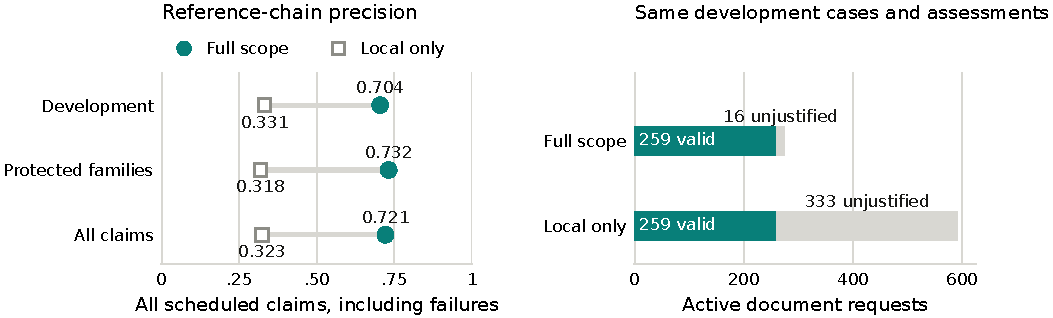
\includegraphics[width=\linewidth]{fig_scope_control.pdf}
\caption{\textbf{Inherited scope removes unjustified demand.} Left:
reference-chain precision in the retrospective current-case evaluation,
including every scheduled case and failure penalty. Right: on the same
\asDevCpN{} completed development cases, both controllers retain
\asDevCpValid{} valid requests; enclosing scope reduces total requests
from \asDevLsReq{} to \asDevCpReq. The assessment and source representation
are fixed.}
\label{fig:scope}
\end{figure}

\paragraph{The benefit is selectivity at fixed assessment.}
Figure~\ref{fig:scope} isolates inherited domain scope: an obligation must
satisfy the enclosing process conditions as well as its local guard.
On protected families, native valid-chain precision rises from
\asHidLsChain{} to \asHidCpChain; the conservative paired benefit remains
positive at \asHidCChain{} even after penalizing unavailable pairs. The
corresponding unnecessary fraction falls from \asHidLsU{} to
\asHidCpU. These are complementary views of the same requests, not
independent effects. On the same \asDevCpN{} completed development cases,
both controllers recover \asDevCpValid{} valid requests, while total
requests fall from \asDevLsReq{} to \asDevCpReq. Scope therefore removes
unjustified demands without sacrificing those recovered obligations.
The compiled-equivalent control matches \casepath exactly. The intervention
establishes the value of inherited domain applicability; it does not isolate
arbitrary graph topology. Native chain matching checks agreement with
reference decision--fact--capability--document links, not exact-source
entailment: provenance-chain inheritance is zero in both controllers.

The family label records the original target-custody split: observable
inputs had been inspected during product work, historical target non-access
is not established because the producer's complete I/O audit is missing,
and targets are now released. These are finite-corpus descriptive analyses,
not fresh hidden confirmation. Costs are \$\nrStudyCost{} for the study and
\$\nrTotalCost{} including earlier activity; the retrospective analyses add
no provider calls. Full endpoints, raw counts and paired contrasts are in
Appendix~\ref{app:request-diagnostic} and Appendix~\ref{app:assessed-state}.
